\newcommand\hilight[2]{\color{#1}#2\color{black}}
\definecolor{grey}{RGB}{127,127,127}
\definecolor{darkcyan}{RGB}{0,127,127}
\definecolor{olivegreen}{RGB}{0,127,0}
\definecolor{violet}{RGB}{127,0,127}
\definecolor{brickred}{RGB}{127,0,0}
\definecolor{brown}{RGB}{127,63,0}
\definecolor{red}{RGB}{127,0,0}

\section{Landslide}
\label{sec:landslide}

Landslide is an experimental tool for helping kernel authors find and debug concurrency errors.
It is based on the technique of systematic exploration~\cite{verisoft}, a way of exploring the state space of different thread interleavings in a concurrent system.
It follows in the footsteps of related tools such as
\shortversion{CHESS~\cite{chess},}
{CHESS~\cite{chess}, dBug~\cite{dbug-ssv}, and DeMeter~\cite{demeter},}
but is the first tool we know of to apply systematic exploration in a kernel development environment.

Conceptually,
Landslide is designed as follows.
Students annotate their code so Landslide knows
which kernel thread is currently running.
After one kernel thread has run for some time,
Landslide triggers artificial clock interrupts
% to force a new thread to interleave with the current one.
to force the scheduler to run a different thread.
When a test program finishes execution according
to one pattern of thread switches,
Landslide rewinds the kernel's state
and resumes the test according to a different thread interleaving.
After each instruction,
Landslide applies several bug-detection predicates to
the kernel's state to detect
illegal heap accesses,
deadlock, infinite loops, and panics.
\shortversion{}{In theory,
by forcing a thread switch after every non-scheduler instruction,
Landslide could apply its bug-detection predicates to every reachable
execution state.
Because this would require prohibitive time to complete,
in practice Landslide uses a variety of techniques to
thread-switch less often and to avoid repeating
bug-equivalent execution paths.}
%Landslide is implemented as a module for Simics, the simulator our students use as an execution environment for their kernels. Simics can load Landslide while booting a student's kernel, and calls into Landslide once per simulated instruction and once per simulated memory access.
%Landslide uses this information to update its internal representation of the kernel's state, which it in turn uses to decide how to control the kernel's execution.

In this section we give an overview of Landslide's design and interface, and point out the annotations students need to provide to make Landslide work with their own code.

%%%%%%%%%%%%%%%%%%%%%%%%%%%%%%%%%%%%%%%%%%%%%%%%%%%%%%%%%%%%%%%%%%%%%%%%%%%%%%%%
\subsection{Example}
% TODO: if necessary, this can be not its own section

Figure~\ref{fig:threadfork} shows code containing a timer-dependent bug common in many Pebbles implementations which we will use as a running example\shortversion{.}{in the rest of this section.}
This code is a simplified implementation of the \x{thread_fork} system call: it constructs data structures necessary for the new thread, then asks the scheduler to make the new thread runnable, then returns its assigned thread ID.
However, if the timer preempts execution at line~\ref{line:hax}, the child thread might run long enough to exit, causing \x{child} to become a dangling pointer.

\begin{figure}[t]
\small
\begin{lstlisting}[numbers=left]
int thread_fork() {
	thread_t *child = construct_new_thread();
	add_to_runqueue(child);
	// at this point child may run and exit#\label{line:hax}#
	return child->tid;#\label{line:owned}#
}
\end{lstlisting}
\caption{Example race condition. If a timer interrupt occurs at line~\ref{line:hax}, the child thread can run, exit, and free its state, causing line~\ref{line:owned}'s access to be a use-after-free.}
\label{fig:threadfork}
\end{figure}

%%%%%%%%%%%%%%%%%%%%%%%%%%%%%%%%%%%%%%%%%%%%%%%%%%%%%%%%%%%%%%%%%%%%%%%%%%%%%%%%
\subsection{Testing Mechanism}

Systematic exploration, Landslide's mechanism for testing many different concurrent scenarios, uses the idea of an {\em execution tree} to enumerate all possible thread interleavings of a specific test. These interleavings are defined around {\em decision points}, which intuitively indicate points during execution at which a preemption could cause different behaviour to arise.
Searching with few decision points results in coarser-grained interleavings, faster test completion, and less likelihood of finding unexpected bugs; searching with more decision points results in the opposite.
The primary advantage of systematic testing is the ability to force execution sequences that might be overlooked in simple stress testing.
% Unlike simple testing, systematic execution reaches all execution states, so it does not overlook rare bugs.

Landslide ``explores'' an execution tree by controlling the kernel's execution in two ways.
First, at each decision point, it can force an arbitary thread to run in place of the current one by injecting timer interrupts to force the kernel to context switch.
%Second, whenever the kernel finishes executing a particular interleaving of the test case, it reverts the system to an earlier state to explore additional interleavings using Simics's reverse execution.
Second, when the kernel finishes executing a particular interleaving of the test case, it invokes Simics reverse execution to revert the system to an earlier state and explore the next interleaving.

In Figure~\ref{fig:threadfork}, the necessary decision point for finding the bug is at line~\ref{line:hax}. With correct instrumentation (discussed in Section~\ref{sec:instrument} and shown in Figure~\ref{fig:annotation}), Landslide can automatically identify this decision point because a thread becomes runnable.
Landslide also automatically identifies decision points at voluntary reschedules between threads (e.g. \x{yield()}). Together these decision points define an execution tree which exposes this bug, depicted in Figure~\ref{fig:tree}.


Of course, additional decision points are often necessary to expose more-subtle race conditions.
% \shortversion
% {In Section~\ref{sec:instrument} we describe an interface for adding new
% decision points to expand the state space,
% and also an interface for restricting Landslide's attention to certain kernel components,
% which helps cope with the exponentially-growing nature of state spaces with many decision points.}
We provide an interface for adding new decision points to expand the state space.
%described in Section~\ref{sec:decision}.
In order to cope with the exponentially-growing nature of state spaces with many decision points,
\shortversion{we also provide an interface for making Landslide consider}
{Landslide uses the Dynamic Partial Order Reduction algorithm~\cite{dpor} to identify and prune redundant thread interleavings, the specifics of which are beyond the scope of this educational work~\cite{landslide}.
We also provide an interface for helping Landslide further reduce the state space by considering}
decision points from only certain components of the kernel.
%which we discuss in Section~\ref{sec:focusing}.
Section~\ref{sec:instrument} discusses these interface options.

\begin{figure}[t]
	\centering
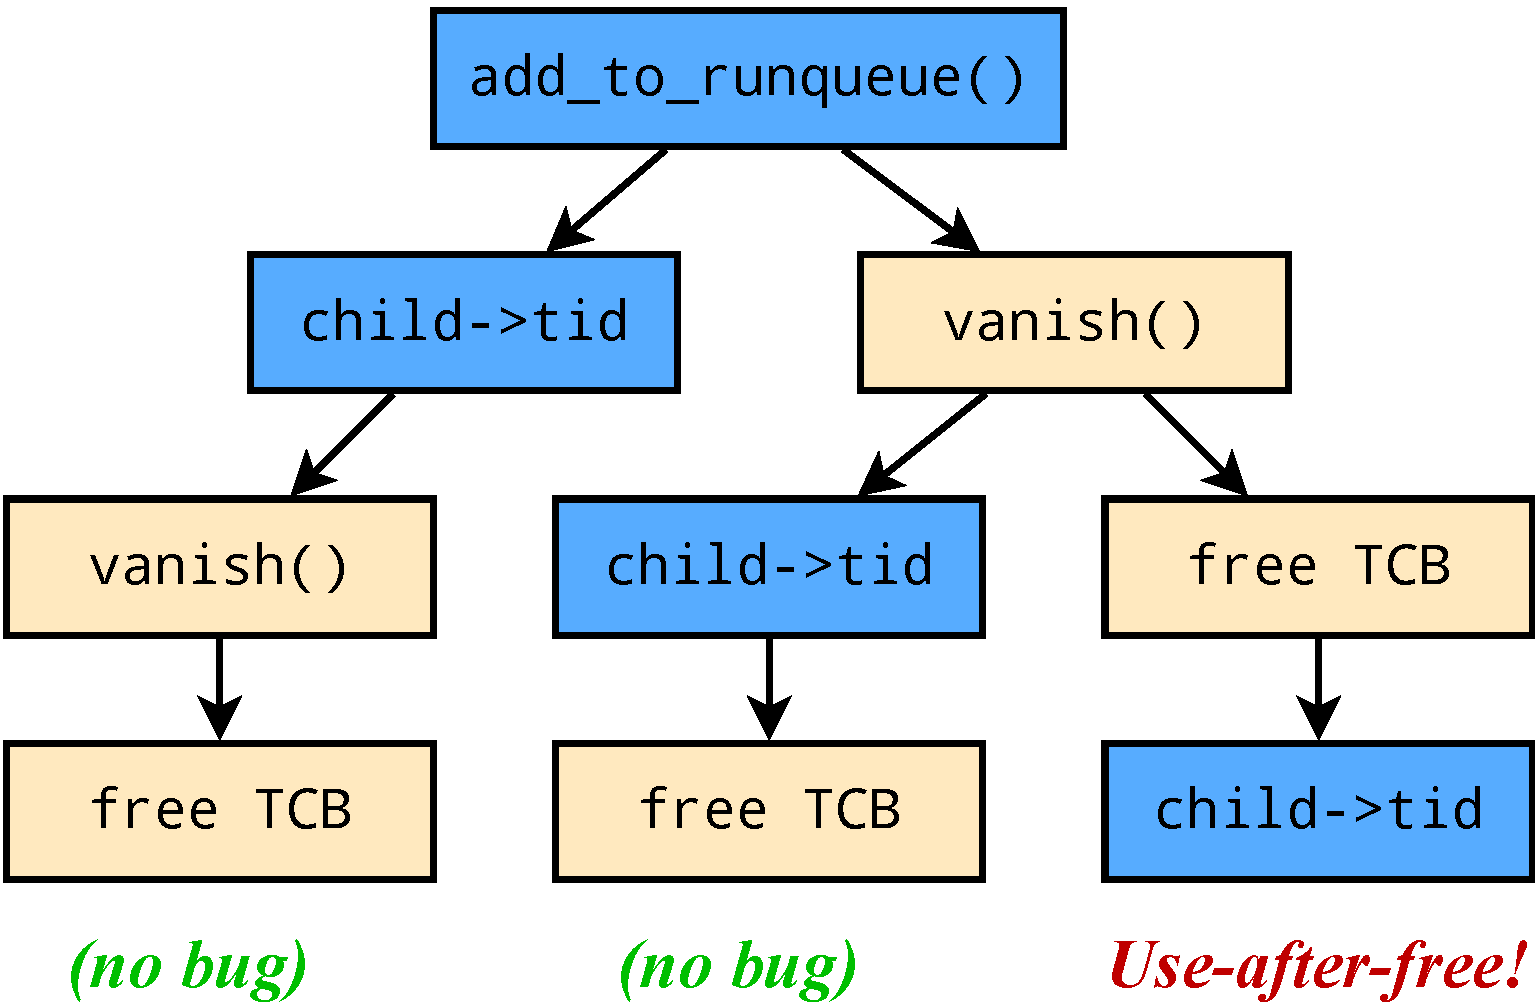
\includegraphics[width=0.42\textwidth]{threadfork/threadfork.pdf}
\caption{The state space of possible thread interleavings can be viewed as an {\em execution tree}.
Landslide uses timer interrupts to force different threads to run as it explores this tree.
If a kernel has concurrency errors, they will show up in some branches, but not others.
This tree shows the bug from Figure~\ref{fig:threadfork}, with operations from the parent thread shaded.
}
\label{fig:tree}
\end{figure}

%%%%%%%%%%%%%%%%%%%%%%%%%%%%%%%%%%%%%%%%%%%%%%%%%%%%%%%%%%%%%%%%%%%%%%%%%%%%%%%%
\subsection{Identifying Bugs}

Landslide has several checks that detect when a bug arises. It can identify kernel panics, use-after-free accesses (and other heap-related errors such as double-free and memory leaks), and
\shortversion{
deadlocks, and also includes a heuristic check for infinite loops and livelock.
}{
deadlocks.
Landslide can optionally also check heuristically for infinite loops and livelock. This is done by comparing the length of the current interleaving against previously-explored ones: if the current interleaving has been running disproportionately longer (by a large arbitrary constant factor), we assume the kernel is stuck.
We have not found this technique to erroneously report false positives, although it may fail to trigger when it ought to if too few previous interleavings have been tested to make a reliable comparison.
}

When Landslide identifies a bug, it outputs a
\shortversion
{{\em decision trace} (Figure~\ref{fig:trace}).}
{{\em decision trace}, an example of which is shown in Figure~\ref{fig:trace}.}
The trace reports what kind of bug was detected
\shortversion
{and}
{(for uses-after-free, it also prints stack traces to show when the block was allocated and freed), and}
also reports each decision point in the current interleaving: which thread was running, a trace of its stack when it was switched away from, and the thread that Landslide caused to preempt it.
With this trace, the student can better understand the concurrent execution that exposed the bug.

Note that our use of the term ``race condition'' throughout this paper refers to concurrency errors in general, a category that includes data races, atomicity violations, and nondeterministic deadlocks.
In contrast with analyses that directly detect data races~\cite{tsan}, Landslide does not identify bugs at suspicious memory accesses, but rather detects failure conditions that can arise from many different types of errors.
\shortversion{}{In general,
% with false-negative bug detection,
a kernel might contain a buggy behaviour that Landslide could overlook (i.e., a false negative). However (except in the case of heuristic infinite loop detection), when Landslide does identify a bug, the student can be sure that an error exists.
}

\newcommand\bug[1]{\hilight{red}{#1}}
\newcommand\decision[1]{\bfseries \hilight{olivegreen}{#1}}
\newcommand\stacktrace[1]{\hilight{darkcyan}{#1}}
\begin{figure}[t]
\small
\begin{lstlisting}
#\bfseries \bug{USE~AFTER~FREE:~read~from~0x15a8f0~at~IP~0x104209}#
#\bug{Block~0x15a8f0~was~allocated~by~thread~3~at~(...)}#
                   #\bug{and~freed~by~thread~4~at~(...)}#
Decision trace follows:
#\decision{1:  switched from thread 3 -> thread 4 at:}#
        0x105a10 in #\stacktrace{context\_switch}#,
        0x1041f4 in #\stacktrace{thread\_fork}#,
        0x10362b in #\stacktrace{thread\_fork\_wrapper}#
#\decision{2:  switched from thread 4 -> thread 3 at:}#
        0x105a10 in #\stacktrace{context\_switch}#,
        0x104681 in #\stacktrace{yield}#,
        0x104570 in #\stacktrace{exit}#,
        0x103708 in #\stacktrace{exit\_wrapper}#
#\decision{Current thread 3 at:}#
        0x104209 in #\stacktrace{thread\_fork}#,
        0x10362b in #\stacktrace{thread\_fork\_wrapper}#
Total decision points 24, total backtracks 5
\end{lstlisting}
\caption{Landslide outputs this trace for Figure~\ref{fig:threadfork}'s bug.}
\label{fig:trace}
\end{figure}

%%%%%%%%%%%%%%%%%%%%%%%%%%%%%%%%%%%%%%%%%%%%%%%%%%%%%%%%%%%%%%%%%%%%%%%%%%%%%%%%
\subsection{Instrumentation}
\label{sec:instrument}

Landslide's interface is comprised of two types of instrumentation which students must provide: {\em required annotations} and {\em configuring decision points}.

\subsubsection{Required annotations}
Users annotate their kernels to inform Landslide of certain important concurrency events during execution. We provide a set of annotation functions, named with the prefix \x{tell_landslide}, for this purpose. The annotations denote when a thread runs \x{fork}, \x{sleep}, or \x{vanish}, when a thread is added to or removed from the runqueue, and when a thread becomes blocked on a mutex.
Figure~\ref{fig:annotation} shows annotated code corresponding to Figure~\ref{fig:threadfork}.

There is also a configuration file, \x{config.landslide}, in which the student must specify constant information such as the function names of the timer handler and context switcher, which threads exist when the kernel boots, and which user-space test program Landslide should invoke.
Finally, there are two short (nominally two-line) functions used within Landslide itself that the user must implement. These are predicates on the kernel's scheduler state, and express potentially nontrivial conditions: whether the current thread is runnable but not on the runqueue, and whether preemption is disabled while interrupts are on.

\newcommand\telllandslide[1]{\bfseries \color{violet}{#1}}
\begin{figure}[t]
\small
\begin{lstlisting}
void add_to_runqueue(thread_t *child) {
	#\telllandslide{tell\_landslide\_thread\_runnable(child->tid);}#
	// ...
}
int thread_fork() {
	thread_t *child = construct_new_thread();
	#\telllandslide{tell\_landslide\_forking(child->tid);}#
	add_to_runqueue(child);
	return child->tid;
}
\end{lstlisting}
\caption{Landslide requires the programmer to annotate important concurrency events\shortversion{.}{in their kernel.} \x{tell_landslide_thread_runnable()} indicates that a thread can henceforth be forced to run with timer interrupts, and \x{tell_landslide_forking()} announces a new thread's existence.}
\label{fig:annotation}
\end{figure}

\subsubsection{Configuring decision points}
\label{sec:decision}

Using only decision points that Landslide automatically identifies on voluntary reschedules will result in coarse-grained interleavings likely to overlook bugs.
We provide an extra annotation
for students to add more decision points for a finer-grained search, called
\x{tell_landslide_decide()}.
We recommend inserting it into concurrency primitives, such as at the start of \x{mutex_lock()} and at the end of \x{mutex_unlock()}.

\subsubsection{Focusing the search space}
\label{sec:focusing}

The strategy we describe above may cause Landslide to identify decision points in unrelated parts of the kernel, such as when accessing mutexes in unrelated and/or already-trusted system calls.
We provide interface options in \x{config.landslide} for the student to view currently identified decision points and to selectively eliminate them.
If a student were testing thread death and reaping, they might want decision points to appear in \x{wait} and \x{vanish} but not if unrelated virtual memory operations are also in progress.
Accordingly, they could write \x{within_function wait vanish} and \x{without_function} \x{destroy_address_space}.
The \x{within_function} directive requires that at least one of the specified functions shall be on the call stack when decision points are identified, and \x{without_function} requires the opposite.

% First, the student writes ``\x{DECISION_INFO_ONLY}'' to make Landslide run only one interleaving and then print all decision points instead of continuing to explore.
% In this file, students can write ``\x{within_function} \x{foo}'' to whitelist function \x{foo}, and ``\x{without_function} \x{bar}'' to blacklist function \x{bar}.
% In this file, students can use the ``\x{within_function}'' and ``\x{without_function}'' directives to require that given functions are or are not on the call stack when decision points are identified.
% make Landslide ignore any decision points that don't arise from the execution of specific functions.
% For example, if testing thread death and reaping, the student should write \x{within_function exit} and \x{within_function} \x{wait}, and also
% (assuming they don't care about the virtual memory operations associated with \x{exit})
% \x{without_function} \x{destroy_address_space}.

% Additionally, the student may configure Landslide's state space reduction to ignore certain memory locations.
% DPOR's analysis requires a memory independence relation between thread transitions; the more transitions are independent from each other, the more reduction can be achieved.
% Unfortunately, in the kernel environment, every thread switch will execute through a common path that modifies shared scheduler data structures.
% Unchecked, this would cause every transition to conflict with each other and result in no reduction in execution time from DPOR.
% Certain other shared memory conflicts also arise that are irrelevant to whichever system calls are being tested; for example, if testing for races in thread lifecycle routines, the user likely does not care about accesses to the frame allocator mutex.
%
% We provide an interface with which the user can configure Landslide to ignore such unrelated conflicts to more efficiently test components of the kernel they care about.
% In \x{config.landslide}, the user writes ``\x{ignore_sym}'' followed by the name of the global variable to ignore and its type size, and Landslide may then identify transitions as independent even if they conflict on that memory.

%%%%%%%%%%%%%%%%%%%%%%%%%%%%%%%%%%%%%%%%%%%%%%%%%%%%%%%%%%%%%%%%%%%%%%%%%%%%%%%%
\subsection{Limitations}

Landslide currently assumes that timer interrupts are the only nondeterministic events that influence a kernel's concurrent execution. While this prevents us from finding races related to external input such as disk or network I/O, Landslide is already able to find many types of complicated races by controlling timer-driven thread scheduling.
Landslide's model is also currently restricted to uniprocessor execution.
Supporting multiprocessor environments and device driver testing is left to future work.
% this used to say ", and production kernels"

In contrast with conventional stress testing, in which the test program exercises many system calls, Landslide works best with very small test cases.
Landslide's coverage results from exploring the different scheduling possibilities that arise from a short sequence of system calls.
If Landslide were used when running a stress test, the resulting state space would be too large to explore feasibly.
Hence, when working with students, we provided a suite of four test programs, each no longer than 10 lines of code, but carefully written to bring about system call interactions known to be troublesome.

